\documentclass[1p]{elsarticle_modified}
%\bibliographystyle{elsarticle-num}

%\usepackage[colorlinks]{hyperref}
%\usepackage{abbrmath_seonhwa} %\Abb, \Ascr, \Acal ,\Abf, \Afrak
\usepackage{amsfonts}
\usepackage{amssymb}
\usepackage{amsmath}
\usepackage{amsthm}
\usepackage{scalefnt}
\usepackage{amsbsy}
\usepackage{kotex}
\usepackage{caption}
\usepackage{subfig}
\usepackage{color}
\usepackage{graphicx}
\usepackage{xcolor} %% white, black, red, green, blue, cyan, magenta, yellow
\usepackage{float}
\usepackage{setspace}
\usepackage{hyperref}

\usepackage{tikz}
\usetikzlibrary{arrows}

\usepackage{multirow}
\usepackage{array} % fixed length table
\usepackage{hhline}

%%%%%%%%%%%%%%%%%%%%%
\makeatletter
\renewcommand*\env@matrix[1][\arraystretch]{%
	\edef\arraystretch{#1}%
	\hskip -\arraycolsep
	\let\@ifnextchar\new@ifnextchar
	\array{*\c@MaxMatrixCols c}}
\makeatother %https://tex.stackexchange.com/questions/14071/how-can-i-increase-the-line-spacing-in-a-matrix
%%%%%%%%%%%%%%%

\usepackage[normalem]{ulem}

\newcommand{\msout}[1]{\ifmmode\text{\sout{\ensuremath{#1}}}\else\sout{#1}\fi}
%SOURCE: \msout is \stkout macro in https://tex.stackexchange.com/questions/20609/strikeout-in-math-mode

\newcommand{\cancel}[1]{
	\ifmmode
	{\color{red}\msout{#1}}
	\else
	{\color{red}\sout{#1}}
	\fi
}

\newcommand{\add}[1]{
	{\color{blue}\uwave{#1}}
}

\newcommand{\replace}[2]{
	\ifmmode
	{\color{red}\msout{#1}}{\color{blue}\uwave{#2}}
	\else
	{\color{red}\sout{#1}}{\color{blue}\uwave{#2}}
	\fi
}

\newcommand{\Sol}{\mathcal{S}} %segment
\newcommand{\D}{D} %diagram
\newcommand{\A}{\mathcal{A}} %arc


%%%%%%%%%%%%%%%%%%%%%%%%%%%%%5 test

\def\sl{\operatorname{\textup{SL}}(2,\Cbb)}
\def\psl{\operatorname{\textup{PSL}}(2,\Cbb)}
\def\quan{\mkern 1mu \triangleright \mkern 1mu}

\theoremstyle{definition}
\newtheorem{thm}{Theorem}[section]
\newtheorem{prop}[thm]{Proposition}
\newtheorem{lem}[thm]{Lemma}
\newtheorem{ques}[thm]{Question}
\newtheorem{cor}[thm]{Corollary}
\newtheorem{defn}[thm]{Definition}
\newtheorem{exam}[thm]{Example}
\newtheorem{rmk}[thm]{Remark}
\newtheorem{alg}[thm]{Algorithm}

\newcommand{\I}{\sqrt{-1}}
\begin{document}

%\begin{frontmatter}
%
%\title{Boundary parabolic representations of knots up to 8 crossings}
%
%%% Group authors per affiliation:
%\author{Yunhi Cho} 
%\address{Department of Mathematics, University of Seoul, Seoul, Korea}
%\ead{yhcho@uos.ac.kr}
%
%
%\author{Seonhwa Kim} %\fnref{s_kim}}
%\address{Center for Geometry and Physics, Institute for Basic Science, Pohang, 37673, Korea}
%\ead{ryeona17@ibs.re.kr}
%
%\author{Hyuk Kim}
%\address{Department of Mathematical Sciences, Seoul National University, Seoul 08826, Korea}
%\ead{hyukkim@snu.ac.kr}
%
%\author{Seokbeom Yoon}
%\address{Department of Mathematical Sciences, Seoul National University, Seoul, 08826,  Korea}
%\ead{sbyoon15@snu.ac.kr}
%
%\begin{abstract}
%We find all boundary parabolic representation of knots up to 8 crossings.
%
%\end{abstract}
%\begin{keyword}
%    \MSC[2010] 57M25 
%\end{keyword}
%
%\end{frontmatter}

%\linenumbers
%\tableofcontents
%
\newcommand\colored[1]{\textcolor{white}{\rule[-0.35ex]{0.8em}{1.4ex}}\kern-0.8em\color{red} #1}%
%\newcommand\colored[1]{\textcolor{white}{ #1}\kern-2.17ex	\textcolor{white}{ #1}\kern-1.81ex	\textcolor{white}{ #1}\kern-2.15ex\color{red}#1	}

{\Large $\underline{12a_{1175}~(K12a_{1175})}$}

\setlength{\tabcolsep}{10pt}
\renewcommand{\arraystretch}{1.6}
\vspace{1cm}\begin{tabular}{m{100pt}>{\centering\arraybackslash}m{274pt}}
\multirow{5}{120pt}{
	\centering
	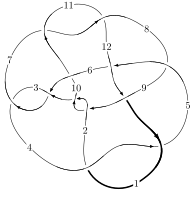
\includegraphics[width=112pt]{../../../GIT/diagram.site/Diagrams/png/1976_12a_1175.png}\\
\ \ \ A knot diagram\footnotemark}&
\allowdisplaybreaks
\textbf{Linearized knot diagam} \\
\cline{2-2}
 &
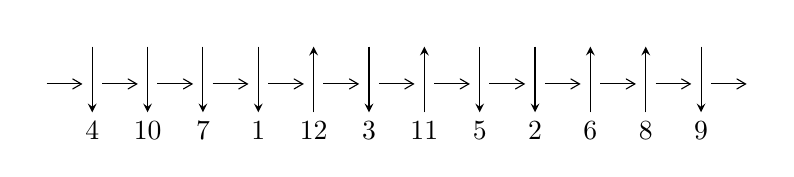
\begin{tikzpicture}[x=20pt, y=17pt]
	% nodes
	\node (C0) at (0, 0) {};
	\node (C1) at (1, 0) {};
	\node (C1U) at (1, +1) {};
	\node (C1D) at (1, -1) {4};

	\node (C2) at (2, 0) {};
	\node (C2U) at (2, +1) {};
	\node (C2D) at (2, -1) {10};

	\node (C3) at (3, 0) {};
	\node (C3U) at (3, +1) {};
	\node (C3D) at (3, -1) {7};

	\node (C4) at (4, 0) {};
	\node (C4U) at (4, +1) {};
	\node (C4D) at (4, -1) {1};

	\node (C5) at (5, 0) {};
	\node (C5U) at (5, +1) {};
	\node (C5D) at (5, -1) {12};

	\node (C6) at (6, 0) {};
	\node (C6U) at (6, +1) {};
	\node (C6D) at (6, -1) {3};

	\node (C7) at (7, 0) {};
	\node (C7U) at (7, +1) {};
	\node (C7D) at (7, -1) {11};

	\node (C8) at (8, 0) {};
	\node (C8U) at (8, +1) {};
	\node (C8D) at (8, -1) {5};

	\node (C9) at (9, 0) {};
	\node (C9U) at (9, +1) {};
	\node (C9D) at (9, -1) {2};

	\node (C10) at (10, 0) {};
	\node (C10U) at (10, +1) {};
	\node (C10D) at (10, -1) {6};

	\node (C11) at (11, 0) {};
	\node (C11U) at (11, +1) {};
	\node (C11D) at (11, -1) {8};

	\node (C12) at (12, 0) {};
	\node (C12U) at (12, +1) {};
	\node (C12D) at (12, -1) {9};
	\node (C13) at (13, 0) {};

	% arrows
	\draw[->,>={angle 60}]
	(C0) edge (C1) (C1) edge (C2) (C2) edge (C3) (C3) edge (C4) (C4) edge (C5) (C5) edge (C6) (C6) edge (C7) (C7) edge (C8) (C8) edge (C9) (C9) edge (C10) (C10) edge (C11) (C11) edge (C12) (C12) edge (C13) ;	\draw[->,>=stealth]
	(C1U) edge (C1D) (C2U) edge (C2D) (C3U) edge (C3D) (C4U) edge (C4D) (C5D) edge (C5U) (C6U) edge (C6D) (C7D) edge (C7U) (C8U) edge (C8D) (C9U) edge (C9D) (C10D) edge (C10U) (C11D) edge (C11U) (C12U) edge (C12D) ;
	\end{tikzpicture} \\
\hhline{~~} \\& 
\textbf{Solving Sequence} \\ \cline{2-2} 
 &
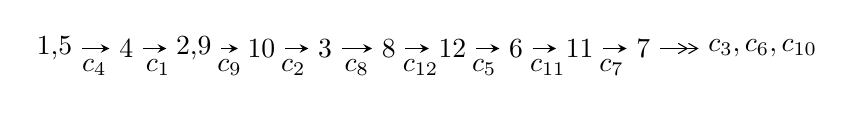
\begin{tikzpicture}[x=23pt, y=7pt]
	% node
	\node (A0) at (-1/8, 0) {1,5};
	\node (A1) at (1, 0) {4};
	\node (A2) at (33/16, 0) {2,9};
	\node (A3) at (25/8, 0) {10};
	\node (A4) at (33/8, 0) {3};
	\node (A5) at (41/8, 0) {8};
	\node (A6) at (49/8, 0) {12};
	\node (A7) at (57/8, 0) {6};
	\node (A8) at (65/8, 0) {11};
	\node (A9) at (73/8, 0) {7};
	\node (C1) at (1/2, -1) {$c_{4}$};
	\node (C2) at (3/2, -1) {$c_{1}$};
	\node (C3) at (21/8, -1) {$c_{9}$};
	\node (C4) at (29/8, -1) {$c_{2}$};
	\node (C5) at (37/8, -1) {$c_{8}$};
	\node (C6) at (45/8, -1) {$c_{12}$};
	\node (C7) at (53/8, -1) {$c_{5}$};
	\node (C8) at (61/8, -1) {$c_{11}$};
	\node (C9) at (69/8, -1) {$c_{7}$};
	\node (A10) at (11, 0) {$c_{3},c_{6},c_{10}$};

	% edge
	\draw[->,>=stealth]	
	(A0) edge (A1) (A1) edge (A2) (A2) edge (A3) (A3) edge (A4) (A4) edge (A5) (A5) edge (A6) (A6) edge (A7) (A7) edge (A8) (A8) edge (A9) ;
	\draw[->>,>={angle 60}]	
	(A9) edge (A10);
\end{tikzpicture} \\ 

\end{tabular} \\

\footnotetext{
The image of knot diagram is generated by the software ``\textbf{Draw programme}" developed by Andrew Bartholomew(\url{http://www.layer8.co.uk/maths/draw/index.htm\#Running-draw}), where we modified some parts for our purpose(\url{https://github.com/CATsTAILs/LinksPainter}).
}\phantom \\ \newline 
\centering \textbf{Ideals for irreducible components\footnotemark of $X_{\text{par}}$} 
 
\begin{align*}
I^u_{1}&=\langle 
5.84939\times10^{910} u^{146}+5.61647\times10^{911} u^{145}+\cdots+2.71478\times10^{912} b-5.72333\times10^{914},\\
\phantom{I^u_{1}}&\phantom{= \langle  }1.06195\times10^{914} u^{146}+8.90133\times10^{914} u^{145}+\cdots+2.22883\times10^{915} a-3.84240\times10^{917},\\
\phantom{I^u_{1}}&\phantom{= \langle  }u^{147}+8 u^{146}+\cdots+61480 u-5747\rangle \\
I^u_{2}&=\langle 
5.49437\times10^{35} u^{35}+2.03279\times10^{36} u^{34}+\cdots+3.20930\times10^{35} b+9.34926\times10^{35},\\
\phantom{I^u_{2}}&\phantom{= \langle  }1.11019\times10^{36} u^{35}+3.24693\times10^{36} u^{34}+\cdots+3.20930\times10^{35} a+4.28373\times10^{36},\;u^{36}+3 u^{35}+\cdots+2 u-1\rangle \\
\\
\end{align*}
\raggedright * 2 irreducible components of $\dim_{\mathbb{C}}=0$, with total 183 representations.\\
\footnotetext{All coefficients of polynomials are rational numbers. But the coefficients are sometimes approximated in decimal forms when there is not enough margin.}
\newpage
\renewcommand{\arraystretch}{1}
\centering \section*{I. $I^u_{1}= \langle 5.85\times10^{910} u^{146}+5.62\times10^{911} u^{145}+\cdots+2.71\times10^{912} b-5.72\times10^{914},\;1.06\times10^{914} u^{146}+8.90\times10^{914} u^{145}+\cdots+2.23\times10^{915} a-3.84\times10^{917},\;u^{147}+8 u^{146}+\cdots+61480 u-5747 \rangle$}
\flushleft \textbf{(i) Arc colorings}\\
\begin{tabular}{m{7pt} m{180pt} m{7pt} m{180pt} }
\flushright $a_{1}=$&$\begin{pmatrix}0\\u\end{pmatrix}$ \\
\flushright $a_{5}=$&$\begin{pmatrix}1\\0\end{pmatrix}$ \\
\flushright $a_{4}=$&$\begin{pmatrix}1\\- u^2\end{pmatrix}$ \\
\flushright $a_{2}=$&$\begin{pmatrix}- u\\u^3+u\end{pmatrix}$ \\
\flushright $a_{9}=$&$\begin{pmatrix}-0.0476460 u^{146}-0.399372 u^{145}+\cdots-1619.95 u+172.395\\-0.0215465 u^{146}-0.206885 u^{145}+\cdots-2194.54 u+210.821\end{pmatrix}$ \\
\flushright $a_{10}=$&$\begin{pmatrix}-0.0733621 u^{146}-0.658696 u^{145}+\cdots-4820.81 u+475.848\\-0.0448746 u^{146}-0.386975 u^{145}+\cdots-2140.92 u+215.379\end{pmatrix}$ \\
\flushright $a_{3}=$&$\begin{pmatrix}0.00620052 u^{146}+0.0524415 u^{145}+\cdots+77.9777 u-11.1646\\-0.00987834 u^{146}-0.0813767 u^{145}+\cdots-269.340 u+32.3155\end{pmatrix}$ \\
\flushright $a_{8}=$&$\begin{pmatrix}-0.0691925 u^{146}-0.606257 u^{145}+\cdots-3814.50 u+383.217\\-0.0215465 u^{146}-0.206885 u^{145}+\cdots-2194.54 u+210.821\end{pmatrix}$ \\
\flushright $a_{12}=$&$\begin{pmatrix}0.0112444 u^{146}+0.140122 u^{145}+\cdots+3100.04 u-285.491\\0.000974400 u^{146}+0.00416042 u^{145}+\cdots-216.608 u+19.9840\end{pmatrix}$ \\
\flushright $a_{6}=$&$\begin{pmatrix}0.0532520 u^{146}+0.349593 u^{145}+\cdots-4377.81 u+370.101\\0.0183596 u^{146}+0.120357 u^{145}+\cdots-1397.64 u+119.695\end{pmatrix}$ \\
\flushright $a_{11}=$&$\begin{pmatrix}0.0144073 u^{146}+0.130613 u^{145}+\cdots+1174.02 u-113.909\\-0.00642001 u^{146}-0.0543650 u^{145}+\cdots-30.5381 u+3.26770\end{pmatrix}$ \\
\flushright $a_{7}=$&$\begin{pmatrix}0.0598125 u^{146}+0.532811 u^{145}+\cdots+3201.29 u-317.212\\0.0375649 u^{146}+0.359767 u^{145}+\cdots+3268.27 u-314.725\end{pmatrix}$\\&\end{tabular}
\flushleft \textbf{(ii) Obstruction class $= -1$}\\~\\
\flushleft \textbf{(iii) Cusp Shapes $= -0.0203121 u^{146}-0.141621 u^{145}+\cdots+1840.41 u-142.702$}\\~\\
\newpage\renewcommand{\arraystretch}{1}
\flushleft \textbf{(iv) u-Polynomials at the component}\newline \\
\begin{tabular}{m{50pt}|m{274pt}}
Crossings & \hspace{64pt}u-Polynomials at each crossing \\
\hline $$\begin{aligned}c_{1},c_{4}\end{aligned}$$&$\begin{aligned}
&u^{147}-8 u^{146}+\cdots+61480 u+5747
\end{aligned}$\\
\hline $$\begin{aligned}c_{2},c_{9}\end{aligned}$$&$\begin{aligned}
&u^{147}-2 u^{146}+\cdots+11046847 u+496609
\end{aligned}$\\
\hline $$\begin{aligned}c_{3},c_{6}\end{aligned}$$&$\begin{aligned}
&u^{147}-3 u^{146}+\cdots+108035 u+24613
\end{aligned}$\\
\hline $$\begin{aligned}c_{5}\end{aligned}$$&$\begin{aligned}
&u^{147}-3 u^{146}+\cdots-73 u-61
\end{aligned}$\\
\hline $$\begin{aligned}c_{7},c_{11}\end{aligned}$$&$\begin{aligned}
&u^{147}-2 u^{146}+\cdots-51044 u+7693
\end{aligned}$\\
\hline $$\begin{aligned}c_{8}\end{aligned}$$&$\begin{aligned}
&u^{147}+6 u^{146}+\cdots-435868 u+78457
\end{aligned}$\\
\hline $$\begin{aligned}c_{10}\end{aligned}$$&$\begin{aligned}
&u^{147}+u^{146}+\cdots+4068286687 u+578211329
\end{aligned}$\\
\hline $$\begin{aligned}c_{12}\end{aligned}$$&$\begin{aligned}
&u^{147}+7 u^{146}+\cdots+24 u-1
\end{aligned}$\\
\hline
\end{tabular}\\~\\
\newpage\renewcommand{\arraystretch}{1}
\flushleft \textbf{(v) Riley Polynomials at the component}\newline \\
\begin{tabular}{m{50pt}|m{274pt}}
Crossings & \hspace{64pt}Riley Polynomials at each crossing \\
\hline $$\begin{aligned}c_{1},c_{4}\end{aligned}$$&$\begin{aligned}
&y^{147}+80 y^{146}+\cdots+2204675628 y-33028009
\end{aligned}$\\
\hline $$\begin{aligned}c_{2},c_{9}\end{aligned}$$&$\begin{aligned}
&y^{147}-110 y^{146}+\cdots+135599578671993 y-246620498881
\end{aligned}$\\
\hline $$\begin{aligned}c_{3},c_{6}\end{aligned}$$&$\begin{aligned}
&y^{147}-83 y^{146}+\cdots+10185969771 y-605799769
\end{aligned}$\\
\hline $$\begin{aligned}c_{5}\end{aligned}$$&$\begin{aligned}
&y^{147}-29 y^{146}+\cdots-148879 y-3721
\end{aligned}$\\
\hline $$\begin{aligned}c_{7},c_{11}\end{aligned}$$&$\begin{aligned}
&y^{147}-104 y^{146}+\cdots+12402263874 y-59182249
\end{aligned}$\\
\hline $$\begin{aligned}c_{8}\end{aligned}$$&$\begin{aligned}
&y^{147}+54 y^{146}+\cdots-169630825840 y-6155500849
\end{aligned}$\\
\hline $$\begin{aligned}c_{10}\end{aligned}$$&$\begin{aligned}
&y^{147}+17 y^{146}+\cdots-2.57\times10^{18} y-3.34\times10^{17}
\end{aligned}$\\
\hline $$\begin{aligned}c_{12}\end{aligned}$$&$\begin{aligned}
&y^{147}+7 y^{146}+\cdots+230 y-1
\end{aligned}$\\
\hline
\end{tabular}\\~\\
\newpage\flushleft \textbf{(vi) Complex Volumes and Cusp Shapes}
$$\begin{array}{c|c|c}  
\text{Solutions to }I^u_{1}& \I (\text{vol} + \sqrt{-1}CS) & \text{Cusp shape}\\
 \hline 
\begin{aligned}
u &= \phantom{-}0.876951 + 0.469338 I \\
a &= -1.034530 - 0.425889 I \\
b &= \phantom{-}0.851366 + 1.024550 I\end{aligned}
 & \phantom{-}0.25753 - 8.60731 I & \phantom{-0.000000 } 0 \\ \hline\begin{aligned}
u &= \phantom{-}0.876951 - 0.469338 I \\
a &= -1.034530 + 0.425889 I \\
b &= \phantom{-}0.851366 - 1.024550 I\end{aligned}
 & \phantom{-}0.25753 + 8.60731 I & \phantom{-0.000000 } 0 \\ \hline\begin{aligned}
u &= -0.169210 + 0.994862 I \\
a &= -1.47924 + 0.45402 I \\
b &= \phantom{-}0.638776 + 0.628243 I\end{aligned}
 & -2.71907 + 3.26464 I & \phantom{-0.000000 } 0 \\ \hline\begin{aligned}
u &= -0.169210 - 0.994862 I \\
a &= -1.47924 - 0.45402 I \\
b &= \phantom{-}0.638776 - 0.628243 I\end{aligned}
 & -2.71907 - 3.26464 I & \phantom{-0.000000 } 0 \\ \hline\begin{aligned}
u &= \phantom{-}0.242383 + 0.952148 I \\
a &= -0.180100 + 0.272064 I \\
b &= \phantom{-}1.51947 + 0.50864 I\end{aligned}
 & \phantom{-}0.73118 - 4.44431 I & \phantom{-0.000000 } 0 \\ \hline\begin{aligned}
u &= \phantom{-}0.242383 - 0.952148 I \\
a &= -0.180100 - 0.272064 I \\
b &= \phantom{-}1.51947 - 0.50864 I\end{aligned}
 & \phantom{-}0.73118 + 4.44431 I & \phantom{-0.000000 } 0 \\ \hline\begin{aligned}
u &= \phantom{-}0.896984 + 0.384069 I \\
a &= \phantom{-}1.005690 - 0.454065 I \\
b &= -0.953019 - 0.568526 I\end{aligned}
 & -1.72980 + 0.90174 I & \phantom{-0.000000 } 0 \\ \hline\begin{aligned}
u &= \phantom{-}0.896984 - 0.384069 I \\
a &= \phantom{-}1.005690 + 0.454065 I \\
b &= -0.953019 + 0.568526 I\end{aligned}
 & -1.72980 - 0.90174 I & \phantom{-0.000000 } 0 \\ \hline\begin{aligned}
u &= \phantom{-}0.102939 + 1.029930 I \\
a &= -1.64929 - 1.29682 I \\
b &= \phantom{-}0.028382 - 0.859907 I\end{aligned}
 & \phantom{-}4.43319 - 2.71551 I & \phantom{-0.000000 } 0 \\ \hline\begin{aligned}
u &= \phantom{-}0.102939 - 1.029930 I \\
a &= -1.64929 + 1.29682 I \\
b &= \phantom{-}0.028382 + 0.859907 I\end{aligned}
 & \phantom{-}4.43319 + 2.71551 I & \phantom{-0.000000 } 0\\
 \hline 
 \end{array}$$\newpage$$\begin{array}{c|c|c}  
\text{Solutions to }I^u_{1}& \I (\text{vol} + \sqrt{-1}CS) & \text{Cusp shape}\\
 \hline 
\begin{aligned}
u &= -0.202073 + 1.028700 I \\
a &= \phantom{-}0.379102 + 0.405956 I \\
b &= -0.296180 - 1.006800 I\end{aligned}
 & -3.83897 - 2.56872 I & \phantom{-0.000000 } 0 \\ \hline\begin{aligned}
u &= -0.202073 - 1.028700 I \\
a &= \phantom{-}0.379102 - 0.405956 I \\
b &= -0.296180 + 1.006800 I\end{aligned}
 & -3.83897 + 2.56872 I & \phantom{-0.000000 } 0 \\ \hline\begin{aligned}
u &= -0.058121 + 0.949008 I \\
a &= -0.11046 + 1.78709 I \\
b &= \phantom{-}0.02723 + 1.57885 I\end{aligned}
 & -4.30862 + 3.41831 I & \phantom{-0.000000 } 0 \\ \hline\begin{aligned}
u &= -0.058121 - 0.949008 I \\
a &= -0.11046 - 1.78709 I \\
b &= \phantom{-}0.02723 - 1.57885 I\end{aligned}
 & -4.30862 - 3.41831 I & \phantom{-0.000000 } 0 \\ \hline\begin{aligned}
u &= -0.400593 + 0.853754 I \\
a &= -0.738910 - 0.221171 I \\
b &= \phantom{-}1.095550 + 0.692165 I\end{aligned}
 & -4.51006 + 0.97799 I & \phantom{-0.000000 } 0 \\ \hline\begin{aligned}
u &= -0.400593 - 0.853754 I \\
a &= -0.738910 + 0.221171 I \\
b &= \phantom{-}1.095550 - 0.692165 I\end{aligned}
 & -4.51006 - 0.97799 I & \phantom{-0.000000 } 0 \\ \hline\begin{aligned}
u &= \phantom{-}0.061534 + 0.938135 I \\
a &= \phantom{-}0.803720 - 0.763167 I \\
b &= -0.87348 - 1.73870 I\end{aligned}
 & \phantom{-}2.53382 - 2.49123 I & \phantom{-0.000000 } 0 \\ \hline\begin{aligned}
u &= \phantom{-}0.061534 - 0.938135 I \\
a &= \phantom{-}0.803720 + 0.763167 I \\
b &= -0.87348 + 1.73870 I\end{aligned}
 & \phantom{-}2.53382 + 2.49123 I & \phantom{-0.000000 } 0 \\ \hline\begin{aligned}
u &= \phantom{-}0.600227 + 0.876715 I \\
a &= \phantom{-}0.115520 - 0.577187 I \\
b &= -0.233182 + 0.146254 I\end{aligned}
 & -1.93708 - 1.02863 I & \phantom{-0.000000 } 0 \\ \hline\begin{aligned}
u &= \phantom{-}0.600227 - 0.876715 I \\
a &= \phantom{-}0.115520 + 0.577187 I \\
b &= -0.233182 - 0.146254 I\end{aligned}
 & -1.93708 + 1.02863 I & \phantom{-0.000000 } 0\\
 \hline 
 \end{array}$$\newpage$$\begin{array}{c|c|c}  
\text{Solutions to }I^u_{1}& \I (\text{vol} + \sqrt{-1}CS) & \text{Cusp shape}\\
 \hline 
\begin{aligned}
u &= \phantom{-}0.930561\phantom{ +0.000000I} \\
a &= \phantom{-}0.758424\phantom{ +0.000000I} \\
b &= -0.477186\phantom{ +0.000000I}\end{aligned}
 & -1.64571\phantom{ +0.000000I} & \phantom{-0.000000 } 0 \\ \hline\begin{aligned}
u &= \phantom{-}0.598023 + 0.898595 I \\
a &= \phantom{-}1.164480 + 0.619413 I \\
b &= -0.595055 - 0.818371 I\end{aligned}
 & \phantom{-}3.39807 - 2.72258 I & \phantom{-0.000000 } 0 \\ \hline\begin{aligned}
u &= \phantom{-}0.598023 - 0.898595 I \\
a &= \phantom{-}1.164480 - 0.619413 I \\
b &= -0.595055 + 0.818371 I\end{aligned}
 & \phantom{-}3.39807 + 2.72258 I & \phantom{-0.000000 } 0 \\ \hline\begin{aligned}
u &= -1.094130 + 0.021306 I \\
a &= \phantom{-}0.948489 + 0.481917 I \\
b &= -0.808507 - 0.654879 I\end{aligned}
 & -9.20594 - 7.28544 I & \phantom{-0.000000 } 0 \\ \hline\begin{aligned}
u &= -1.094130 - 0.021306 I \\
a &= \phantom{-}0.948489 - 0.481917 I \\
b &= -0.808507 + 0.654879 I\end{aligned}
 & -9.20594 + 7.28544 I & \phantom{-0.000000 } 0 \\ \hline\begin{aligned}
u &= \phantom{-}0.893073 + 0.115015 I \\
a &= -1.217280 - 0.253669 I \\
b &= \phantom{-}0.719668 + 0.815559 I\end{aligned}
 & -4.72484 - 2.71448 I & \phantom{-0.000000 } 0 \\ \hline\begin{aligned}
u &= \phantom{-}0.893073 - 0.115015 I \\
a &= -1.217280 + 0.253669 I \\
b &= \phantom{-}0.719668 - 0.815559 I\end{aligned}
 & -4.72484 + 2.71448 I & \phantom{-0.000000 } 0 \\ \hline\begin{aligned}
u &= -0.187421 + 1.097440 I \\
a &= \phantom{-}1.30604 - 1.17317 I \\
b &= \phantom{-}0.072765 - 0.828993 I\end{aligned}
 & \phantom{-}1.10897 + 10.17800 I & \phantom{-0.000000 } 0 \\ \hline\begin{aligned}
u &= -0.187421 - 1.097440 I \\
a &= \phantom{-}1.30604 + 1.17317 I \\
b &= \phantom{-}0.072765 + 0.828993 I\end{aligned}
 & \phantom{-}1.10897 - 10.17800 I & \phantom{-0.000000 } 0 \\ \hline\begin{aligned}
u &= -0.179249 + 1.101150 I \\
a &= -0.591089 + 0.955092 I \\
b &= -0.242870 + 0.945429 I\end{aligned}
 & \phantom{-}4.11202 + 2.41393 I & \phantom{-0.000000 } 0\\
 \hline 
 \end{array}$$\newpage$$\begin{array}{c|c|c}  
\text{Solutions to }I^u_{1}& \I (\text{vol} + \sqrt{-1}CS) & \text{Cusp shape}\\
 \hline 
\begin{aligned}
u &= -0.179249 - 1.101150 I \\
a &= -0.591089 - 0.955092 I \\
b &= -0.242870 - 0.945429 I\end{aligned}
 & \phantom{-}4.11202 - 2.41393 I & \phantom{-0.000000 } 0 \\ \hline\begin{aligned}
u &= -0.156078 + 1.107690 I \\
a &= \phantom{-}0.836814 + 0.411960 I \\
b &= -0.530807 + 0.949615 I\end{aligned}
 & \phantom{-}3.28339 - 0.12770 I & \phantom{-0.000000 } 0 \\ \hline\begin{aligned}
u &= -0.156078 - 1.107690 I \\
a &= \phantom{-}0.836814 - 0.411960 I \\
b &= -0.530807 - 0.949615 I\end{aligned}
 & \phantom{-}3.28339 + 0.12770 I & \phantom{-0.000000 } 0 \\ \hline\begin{aligned}
u &= \phantom{-}0.042875 + 0.874045 I \\
a &= \phantom{-}1.90713 + 0.24861 I \\
b &= -0.588240 + 0.918261 I\end{aligned}
 & \phantom{-}3.76867 + 1.96043 I & \phantom{-0.000000 } 0 \\ \hline\begin{aligned}
u &= \phantom{-}0.042875 - 0.874045 I \\
a &= \phantom{-}1.90713 - 0.24861 I \\
b &= -0.588240 - 0.918261 I\end{aligned}
 & \phantom{-}3.76867 - 1.96043 I & \phantom{-0.000000 } 0 \\ \hline\begin{aligned}
u &= -0.417159 + 1.047950 I \\
a &= \phantom{-}0.299074 + 0.140133 I \\
b &= -1.19668 - 0.87425 I\end{aligned}
 & -5.56249 + 5.90122 I & \phantom{-0.000000 } 0 \\ \hline\begin{aligned}
u &= -0.417159 - 1.047950 I \\
a &= \phantom{-}0.299074 - 0.140133 I \\
b &= -1.19668 + 0.87425 I\end{aligned}
 & -5.56249 - 5.90122 I & \phantom{-0.000000 } 0 \\ \hline\begin{aligned}
u &= -0.185789 + 1.114000 I \\
a &= -1.106120 - 0.671426 I \\
b &= \phantom{-}0.731886 - 1.071050 I\end{aligned}
 & \phantom{-}2.38368 + 3.23403 I & \phantom{-0.000000 } 0 \\ \hline\begin{aligned}
u &= -0.185789 - 1.114000 I \\
a &= -1.106120 + 0.671426 I \\
b &= \phantom{-}0.731886 + 1.071050 I\end{aligned}
 & \phantom{-}2.38368 - 3.23403 I & \phantom{-0.000000 } 0 \\ \hline\begin{aligned}
u &= -0.072876 + 1.144390 I \\
a &= -0.815391 - 0.632412 I \\
b &= \phantom{-}1.02596 - 1.49700 I\end{aligned}
 & \phantom{-}2.77497 + 4.12483 I & \phantom{-0.000000 } 0\\
 \hline 
 \end{array}$$\newpage$$\begin{array}{c|c|c}  
\text{Solutions to }I^u_{1}& \I (\text{vol} + \sqrt{-1}CS) & \text{Cusp shape}\\
 \hline 
\begin{aligned}
u &= -0.072876 - 1.144390 I \\
a &= -0.815391 + 0.632412 I \\
b &= \phantom{-}1.02596 + 1.49700 I\end{aligned}
 & \phantom{-}2.77497 - 4.12483 I & \phantom{-0.000000 } 0 \\ \hline\begin{aligned}
u &= -0.917208 + 0.691962 I \\
a &= -0.660072 - 0.639637 I \\
b &= \phantom{-}1.05527 - 0.97105 I\end{aligned}
 & -4.34907 - 5.78532 I & \phantom{-0.000000 } 0 \\ \hline\begin{aligned}
u &= -0.917208 - 0.691962 I \\
a &= -0.660072 + 0.639637 I \\
b &= \phantom{-}1.05527 + 0.97105 I\end{aligned}
 & -4.34907 + 5.78532 I & \phantom{-0.000000 } 0 \\ \hline\begin{aligned}
u &= -0.292839 + 0.778068 I \\
a &= -0.31649 - 1.74613 I \\
b &= \phantom{-}0.241986 - 1.050730 I\end{aligned}
 & -4.93078 + 2.17996 I & \phantom{-0.000000 } 0 \\ \hline\begin{aligned}
u &= -0.292839 - 0.778068 I \\
a &= -0.31649 + 1.74613 I \\
b &= \phantom{-}0.241986 + 1.050730 I\end{aligned}
 & -4.93078 - 2.17996 I & \phantom{-0.000000 } 0 \\ \hline\begin{aligned}
u &= \phantom{-}0.514617 + 1.052430 I \\
a &= \phantom{-}0.571008 - 0.326610 I \\
b &= -1.275220 + 0.149157 I\end{aligned}
 & \phantom{-}0.36156 - 5.92102 I & \phantom{-0.000000 } 0 \\ \hline\begin{aligned}
u &= \phantom{-}0.514617 - 1.052430 I \\
a &= \phantom{-}0.571008 + 0.326610 I \\
b &= -1.275220 - 0.149157 I\end{aligned}
 & \phantom{-}0.36156 + 5.92102 I & \phantom{-0.000000 } 0 \\ \hline\begin{aligned}
u &= -0.035844 + 0.826571 I \\
a &= \phantom{-}1.89667 - 1.26211 I \\
b &= -0.347194 - 0.690544 I\end{aligned}
 & -3.58582 - 2.05989 I & \phantom{-0.000000 } 0 \\ \hline\begin{aligned}
u &= -0.035844 - 0.826571 I \\
a &= \phantom{-}1.89667 + 1.26211 I \\
b &= -0.347194 + 0.690544 I\end{aligned}
 & -3.58582 + 2.05989 I & \phantom{-0.000000 } 0 \\ \hline\begin{aligned}
u &= \phantom{-}1.174280 + 0.031064 I \\
a &= \phantom{-}0.731603 - 0.530394 I \\
b &= -0.708208 + 1.015300 I\end{aligned}
 & -0.42978 + 6.80664 I & \phantom{-0.000000 } 0\\
 \hline 
 \end{array}$$\newpage$$\begin{array}{c|c|c}  
\text{Solutions to }I^u_{1}& \I (\text{vol} + \sqrt{-1}CS) & \text{Cusp shape}\\
 \hline 
\begin{aligned}
u &= \phantom{-}1.174280 - 0.031064 I \\
a &= \phantom{-}0.731603 + 0.530394 I \\
b &= -0.708208 - 1.015300 I\end{aligned}
 & -0.42978 - 6.80664 I & \phantom{-0.000000 } 0 \\ \hline\begin{aligned}
u &= -0.628690 + 1.011720 I \\
a &= -0.515365 - 0.264585 I \\
b &= \phantom{-}1.62562 + 0.14551 I\end{aligned}
 & -3.22183 + 11.49500 I & \phantom{-0.000000 } 0 \\ \hline\begin{aligned}
u &= -0.628690 - 1.011720 I \\
a &= -0.515365 + 0.264585 I \\
b &= \phantom{-}1.62562 - 0.14551 I\end{aligned}
 & -3.22183 - 11.49500 I & \phantom{-0.000000 } 0 \\ \hline\begin{aligned}
u &= \phantom{-}0.454783 + 1.108180 I \\
a &= -0.264591 + 0.167726 I \\
b &= \phantom{-}0.827780 - 0.453215 I\end{aligned}
 & -1.71882 - 2.08226 I & \phantom{-0.000000 } 0 \\ \hline\begin{aligned}
u &= \phantom{-}0.454783 - 1.108180 I \\
a &= -0.264591 - 0.167726 I \\
b &= \phantom{-}0.827780 + 0.453215 I\end{aligned}
 & -1.71882 + 2.08226 I & \phantom{-0.000000 } 0 \\ \hline\begin{aligned}
u &= \phantom{-}0.770889\phantom{ +0.000000I} \\
a &= -0.372602\phantom{ +0.000000I} \\
b &= \phantom{-}0.649394\phantom{ +0.000000I}\end{aligned}
 & -1.42928\phantom{ +0.000000I} & \phantom{-0.000000 } 0 \\ \hline\begin{aligned}
u &= \phantom{-}0.078790 + 1.253800 I \\
a &= \phantom{-}0.722169 + 0.771577 I \\
b &= -0.067686 + 1.009750 I\end{aligned}
 & \phantom{-}4.52687 - 0.28955 I & \phantom{-0.000000 } 0 \\ \hline\begin{aligned}
u &= \phantom{-}0.078790 - 1.253800 I \\
a &= \phantom{-}0.722169 - 0.771577 I \\
b &= -0.067686 - 1.009750 I\end{aligned}
 & \phantom{-}4.52687 + 0.28955 I & \phantom{-0.000000 } 0 \\ \hline\begin{aligned}
u &= -1.154960 + 0.507268 I \\
a &= -0.312798 - 0.749951 I \\
b &= \phantom{-}0.508256 + 0.770405 I\end{aligned}
 & -5.59782 - 1.30358 I & \phantom{-0.000000 } 0 \\ \hline\begin{aligned}
u &= -1.154960 - 0.507268 I \\
a &= -0.312798 + 0.749951 I \\
b &= \phantom{-}0.508256 - 0.770405 I\end{aligned}
 & -5.59782 + 1.30358 I & \phantom{-0.000000 } 0\\
 \hline 
 \end{array}$$\newpage$$\begin{array}{c|c|c}  
\text{Solutions to }I^u_{1}& \I (\text{vol} + \sqrt{-1}CS) & \text{Cusp shape}\\
 \hline 
\begin{aligned}
u &= \phantom{-}0.468048 + 1.185170 I \\
a &= -0.645720 + 0.382909 I \\
b &= \phantom{-}0.769112 + 1.137780 I\end{aligned}
 & \phantom{-}1.99518 - 4.41462 I & \phantom{-0.000000 } 0 \\ \hline\begin{aligned}
u &= \phantom{-}0.468048 - 1.185170 I \\
a &= -0.645720 - 0.382909 I \\
b &= \phantom{-}0.769112 - 1.137780 I\end{aligned}
 & \phantom{-}1.99518 + 4.41462 I & \phantom{-0.000000 } 0 \\ \hline\begin{aligned}
u &= -0.365267 + 1.225470 I \\
a &= \phantom{-}1.070730 + 0.548707 I \\
b &= -0.77496 + 1.41354 I\end{aligned}
 & \phantom{-}7.68881 + 8.11256 I & \phantom{-0.000000 } 0 \\ \hline\begin{aligned}
u &= -0.365267 - 1.225470 I \\
a &= \phantom{-}1.070730 - 0.548707 I \\
b &= -0.77496 - 1.41354 I\end{aligned}
 & \phantom{-}7.68881 - 8.11256 I & \phantom{-0.000000 } 0 \\ \hline\begin{aligned}
u &= -0.058843 + 0.710421 I \\
a &= \phantom{-}0.110257 + 0.636300 I \\
b &= -1.076690 + 0.456778 I\end{aligned}
 & \phantom{-}2.75824 + 0.94900 I & \phantom{-0.000000 } 0 \\ \hline\begin{aligned}
u &= -0.058843 - 0.710421 I \\
a &= \phantom{-}0.110257 - 0.636300 I \\
b &= -1.076690 - 0.456778 I\end{aligned}
 & \phantom{-}2.75824 - 0.94900 I & \phantom{-0.000000 } 0 \\ \hline\begin{aligned}
u &= \phantom{-}0.254160 + 1.262070 I \\
a &= \phantom{-}1.038250 - 0.416531 I \\
b &= -1.078240 - 0.810680 I\end{aligned}
 & \phantom{-}0.82952 - 5.79904 I & \phantom{-0.000000 } 0 \\ \hline\begin{aligned}
u &= \phantom{-}0.254160 - 1.262070 I \\
a &= \phantom{-}1.038250 + 0.416531 I \\
b &= -1.078240 + 0.810680 I\end{aligned}
 & \phantom{-}0.82952 + 5.79904 I & \phantom{-0.000000 } 0 \\ \hline\begin{aligned}
u &= \phantom{-}0.544422 + 0.455781 I \\
a &= -0.616904 + 0.358057 I \\
b &= \phantom{-}1.65097 + 0.64066 I\end{aligned}
 & -0.607696 + 1.062650 I & \phantom{-0.000000 } 0 \\ \hline\begin{aligned}
u &= \phantom{-}0.544422 - 0.455781 I \\
a &= -0.616904 - 0.358057 I \\
b &= \phantom{-}1.65097 - 0.64066 I\end{aligned}
 & -0.607696 - 1.062650 I & \phantom{-0.000000 } 0\\
 \hline 
 \end{array}$$\newpage$$\begin{array}{c|c|c}  
\text{Solutions to }I^u_{1}& \I (\text{vol} + \sqrt{-1}CS) & \text{Cusp shape}\\
 \hline 
\begin{aligned}
u &= -0.392218 + 1.234100 I \\
a &= \phantom{-}1.35293 + 0.81474 I \\
b &= -0.513121 + 0.786595 I\end{aligned}
 & -4.43472 + 1.08434 I & \phantom{-0.000000 } 0 \\ \hline\begin{aligned}
u &= -0.392218 - 1.234100 I \\
a &= \phantom{-}1.35293 - 0.81474 I \\
b &= -0.513121 - 0.786595 I\end{aligned}
 & -4.43472 - 1.08434 I & \phantom{-0.000000 } 0 \\ \hline\begin{aligned}
u &= \phantom{-}0.134815 + 1.288280 I \\
a &= -1.063060 + 0.845144 I \\
b &= \phantom{-}0.023499 + 0.757121 I\end{aligned}
 & \phantom{-}7.48550 - 0.30234 I & \phantom{-0.000000 } 0 \\ \hline\begin{aligned}
u &= \phantom{-}0.134815 - 1.288280 I \\
a &= -1.063060 - 0.845144 I \\
b &= \phantom{-}0.023499 - 0.757121 I\end{aligned}
 & \phantom{-}7.48550 + 0.30234 I & \phantom{-0.000000 } 0 \\ \hline\begin{aligned}
u &= \phantom{-}0.129168 + 1.293520 I \\
a &= -0.0344937 + 0.1283280 I \\
b &= -0.443884 + 1.279780 I\end{aligned}
 & \phantom{-}3.59604 + 1.41572 I & \phantom{-0.000000 } 0 \\ \hline\begin{aligned}
u &= \phantom{-}0.129168 - 1.293520 I \\
a &= -0.0344937 - 0.1283280 I \\
b &= -0.443884 - 1.279780 I\end{aligned}
 & \phantom{-}3.59604 - 1.41572 I & \phantom{-0.000000 } 0 \\ \hline\begin{aligned}
u &= -0.224277 + 1.282390 I \\
a &= -1.42949 - 0.90486 I \\
b &= \phantom{-}0.515504 - 0.396117 I\end{aligned}
 & -2.10216 + 4.13299 I & \phantom{-0.000000 } 0 \\ \hline\begin{aligned}
u &= -0.224277 - 1.282390 I \\
a &= -1.42949 + 0.90486 I \\
b &= \phantom{-}0.515504 + 0.396117 I\end{aligned}
 & -2.10216 - 4.13299 I & \phantom{-0.000000 } 0 \\ \hline\begin{aligned}
u &= \phantom{-}0.466994 + 1.222470 I \\
a &= \phantom{-}0.752734 - 0.579516 I \\
b &= -0.74668 - 1.67540 I\end{aligned}
 & \phantom{-}5.39069 - 5.56331 I & \phantom{-0.000000 } 0 \\ \hline\begin{aligned}
u &= \phantom{-}0.466994 - 1.222470 I \\
a &= \phantom{-}0.752734 + 0.579516 I \\
b &= -0.74668 + 1.67540 I\end{aligned}
 & \phantom{-}5.39069 + 5.56331 I & \phantom{-0.000000 } 0\\
 \hline 
 \end{array}$$\newpage$$\begin{array}{c|c|c}  
\text{Solutions to }I^u_{1}& \I (\text{vol} + \sqrt{-1}CS) & \text{Cusp shape}\\
 \hline 
\begin{aligned}
u &= -0.689909 + 0.018633 I \\
a &= \phantom{-}0.627722 + 1.195240 I \\
b &= -0.640424 - 0.974324 I\end{aligned}
 & \phantom{-}4.08112 - 4.28867 I & \phantom{-0.000000 } 0 \\ \hline\begin{aligned}
u &= -0.689909 - 0.018633 I \\
a &= \phantom{-}0.627722 - 1.195240 I \\
b &= -0.640424 + 0.974324 I\end{aligned}
 & \phantom{-}4.08112 + 4.28867 I & \phantom{-0.000000 } 0 \\ \hline\begin{aligned}
u &= -1.112310 + 0.693160 I \\
a &= -0.490535 + 0.349355 I \\
b &= \phantom{-}0.895156 - 0.775499 I\end{aligned}
 & -1.58290 - 2.49840 I & \phantom{-0.000000 } 0 \\ \hline\begin{aligned}
u &= -1.112310 - 0.693160 I \\
a &= -0.490535 - 0.349355 I \\
b &= \phantom{-}0.895156 + 0.775499 I\end{aligned}
 & -1.58290 + 2.49840 I & \phantom{-0.000000 } 0 \\ \hline\begin{aligned}
u &= \phantom{-}0.685620 + 1.137660 I \\
a &= -0.922510 - 0.559626 I \\
b &= -0.047576 + 0.816722 I\end{aligned}
 & \phantom{-}4.23284 - 2.62278 I & \phantom{-0.000000 } 0 \\ \hline\begin{aligned}
u &= \phantom{-}0.685620 - 1.137660 I \\
a &= -0.922510 + 0.559626 I \\
b &= -0.047576 - 0.816722 I\end{aligned}
 & \phantom{-}4.23284 + 2.62278 I & \phantom{-0.000000 } 0 \\ \hline\begin{aligned}
u &= -0.337289 + 1.285940 I \\
a &= -0.830160 - 0.004283 I \\
b &= -0.047814 - 0.870643 I\end{aligned}
 & \phantom{-}8.02539 - 0.41935 I & \phantom{-0.000000 } 0 \\ \hline\begin{aligned}
u &= -0.337289 - 1.285940 I \\
a &= -0.830160 + 0.004283 I \\
b &= -0.047814 + 0.870643 I\end{aligned}
 & \phantom{-}8.02539 + 0.41935 I & \phantom{-0.000000 } 0 \\ \hline\begin{aligned}
u &= \phantom{-}1.320310 + 0.240780 I \\
a &= -0.208873 + 0.441659 I \\
b &= \phantom{-}0.611708 - 0.680658 I\end{aligned}
 & \phantom{-}0.180238 + 0.465413 I & \phantom{-0.000000 } 0 \\ \hline\begin{aligned}
u &= \phantom{-}1.320310 - 0.240780 I \\
a &= -0.208873 - 0.441659 I \\
b &= \phantom{-}0.611708 + 0.680658 I\end{aligned}
 & \phantom{-}0.180238 - 0.465413 I & \phantom{-0.000000 } 0\\
 \hline 
 \end{array}$$\newpage$$\begin{array}{c|c|c}  
\text{Solutions to }I^u_{1}& \I (\text{vol} + \sqrt{-1}CS) & \text{Cusp shape}\\
 \hline 
\begin{aligned}
u &= -0.267828 + 1.316030 I \\
a &= -0.719672 - 0.684494 I \\
b &= \phantom{-}0.64805 - 1.65046 I\end{aligned}
 & \phantom{-}4.77198 + 0.83961 I & \phantom{-0.000000 } 0 \\ \hline\begin{aligned}
u &= -0.267828 - 1.316030 I \\
a &= -0.719672 + 0.684494 I \\
b &= \phantom{-}0.64805 + 1.65046 I\end{aligned}
 & \phantom{-}4.77198 - 0.83961 I & \phantom{-0.000000 } 0 \\ \hline\begin{aligned}
u &= -0.424786 + 0.496437 I \\
a &= \phantom{-}1.16223 + 1.35492 I \\
b &= -0.399878 + 1.352760 I\end{aligned}
 & -7.40262 - 2.17728 I & \phantom{-0.000000 } 0 \\ \hline\begin{aligned}
u &= -0.424786 - 0.496437 I \\
a &= \phantom{-}1.16223 - 1.35492 I \\
b &= -0.399878 - 1.352760 I\end{aligned}
 & -7.40262 + 2.17728 I & \phantom{-0.000000 } 0 \\ \hline\begin{aligned}
u &= -0.038537 + 0.645768 I \\
a &= -2.04459 + 0.59487 I \\
b &= \phantom{-}0.758645 + 1.052500 I\end{aligned}
 & -0.60483 - 8.80157 I & \phantom{-0.000000 -}0. + 5.91511 I \\ \hline\begin{aligned}
u &= -0.038537 - 0.645768 I \\
a &= -2.04459 - 0.59487 I \\
b &= \phantom{-}0.758645 - 1.052500 I\end{aligned}
 & -0.60483 + 8.80157 I & \phantom{-0.000000 } 0. - 5.91511 I \\ \hline\begin{aligned}
u &= -0.646035 + 1.196380 I \\
a &= -1.199700 - 0.219788 I \\
b &= \phantom{-}0.791908 - 1.085050 I\end{aligned}
 & -3.18263 + 7.65952 I & \phantom{-0.000000 } 0 \\ \hline\begin{aligned}
u &= -0.646035 - 1.196380 I \\
a &= -1.199700 + 0.219788 I \\
b &= \phantom{-}0.791908 + 1.085050 I\end{aligned}
 & -3.18263 - 7.65952 I & \phantom{-0.000000 } 0 \\ \hline\begin{aligned}
u &= \phantom{-}0.432649 + 1.294050 I \\
a &= \phantom{-}0.974867 - 0.393157 I \\
b &= -0.644214 - 0.814276 I\end{aligned}
 & \phantom{-}2.41235 - 4.82981 I & \phantom{-0.000000 } 0 \\ \hline\begin{aligned}
u &= \phantom{-}0.432649 - 1.294050 I \\
a &= \phantom{-}0.974867 + 0.393157 I \\
b &= -0.644214 + 0.814276 I\end{aligned}
 & \phantom{-}2.41235 + 4.82981 I & \phantom{-0.000000 } 0\\
 \hline 
 \end{array}$$\newpage$$\begin{array}{c|c|c}  
\text{Solutions to }I^u_{1}& \I (\text{vol} + \sqrt{-1}CS) & \text{Cusp shape}\\
 \hline 
\begin{aligned}
u &= \phantom{-}0.010834 + 1.372280 I \\
a &= \phantom{-}0.844158 + 0.823308 I \\
b &= \phantom{-}0.019363 + 0.733749 I\end{aligned}
 & \phantom{-}5.75531 - 4.81060 I & \phantom{-0.000000 } 0 \\ \hline\begin{aligned}
u &= \phantom{-}0.010834 - 1.372280 I \\
a &= \phantom{-}0.844158 - 0.823308 I \\
b &= \phantom{-}0.019363 - 0.733749 I\end{aligned}
 & \phantom{-}5.75531 + 4.81060 I & \phantom{-0.000000 } 0 \\ \hline\begin{aligned}
u &= -0.521815 + 0.272355 I \\
a &= \phantom{-}1.74165 + 1.72169 I \\
b &= -0.299454 - 0.648905 I\end{aligned}
 & -7.59186 + 2.72138 I & -12.80013 - 2.70423 I \\ \hline\begin{aligned}
u &= -0.521815 - 0.272355 I \\
a &= \phantom{-}1.74165 - 1.72169 I \\
b &= -0.299454 + 0.648905 I\end{aligned}
 & -7.59186 - 2.72138 I & -12.80013 + 2.70423 I \\ \hline\begin{aligned}
u &= \phantom{-}0.38337 + 1.36632 I \\
a &= -0.927977 + 0.531607 I \\
b &= \phantom{-}0.86865 + 1.45809 I\end{aligned}
 & \phantom{-}5.65267 - 12.88380 I & \phantom{-0.000000 } 0 \\ \hline\begin{aligned}
u &= \phantom{-}0.38337 - 1.36632 I \\
a &= -0.927977 - 0.531607 I \\
b &= \phantom{-}0.86865 - 1.45809 I\end{aligned}
 & \phantom{-}5.65267 + 12.88380 I & \phantom{-0.000000 } 0 \\ \hline\begin{aligned}
u &= \phantom{-}0.334531 + 0.468970 I \\
a &= -0.675876 - 0.038492 I \\
b &= -0.800093 + 0.731056 I\end{aligned}
 & \phantom{-}2.85205 + 0.91488 I & -0.94274 + 1.15824 I \\ \hline\begin{aligned}
u &= \phantom{-}0.334531 - 0.468970 I \\
a &= -0.675876 + 0.038492 I \\
b &= -0.800093 - 0.731056 I\end{aligned}
 & \phantom{-}2.85205 - 0.91488 I & -0.94274 - 1.15824 I \\ \hline\begin{aligned}
u &= \phantom{-}0.45026 + 1.35340 I \\
a &= -1.060430 + 0.679635 I \\
b &= \phantom{-}0.669703 + 1.023420 I\end{aligned}
 & -0.19042 - 7.55699 I & \phantom{-0.000000 } 0 \\ \hline\begin{aligned}
u &= \phantom{-}0.45026 - 1.35340 I \\
a &= -1.060430 - 0.679635 I \\
b &= \phantom{-}0.669703 - 1.023420 I\end{aligned}
 & -0.19042 + 7.55699 I & \phantom{-0.000000 } 0\\
 \hline 
 \end{array}$$\newpage$$\begin{array}{c|c|c}  
\text{Solutions to }I^u_{1}& \I (\text{vol} + \sqrt{-1}CS) & \text{Cusp shape}\\
 \hline 
\begin{aligned}
u &= \phantom{-}0.528484 + 0.213035 I \\
a &= \phantom{-}1.75800 + 0.90834 I \\
b &= -0.683018 - 0.472616 I\end{aligned}
 & -3.45760 - 2.92189 I & -11.27209 + 7.45409 I \\ \hline\begin{aligned}
u &= \phantom{-}0.528484 - 0.213035 I \\
a &= \phantom{-}1.75800 - 0.90834 I \\
b &= -0.683018 + 0.472616 I\end{aligned}
 & -3.45760 + 2.92189 I & -11.27209 - 7.45409 I \\ \hline\begin{aligned}
u &= -0.561562\phantom{ +0.000000I} \\
a &= \phantom{-}0.787362\phantom{ +0.000000I} \\
b &= -2.09875\phantom{ +0.000000I}\end{aligned}
 & \phantom{-}0.814544\phantom{ +0.000000I} & -30.4670\phantom{ +0.000000I} \\ \hline\begin{aligned}
u &= -1.44077 + 0.01593 I \\
a &= -0.587519 + 0.383106 I \\
b &= \phantom{-}0.858394 - 0.944654 I\end{aligned}
 & -4.23476 + 12.61430 I & \phantom{-0.000000 } 0 \\ \hline\begin{aligned}
u &= -1.44077 - 0.01593 I \\
a &= -0.587519 - 0.383106 I \\
b &= \phantom{-}0.858394 + 0.944654 I\end{aligned}
 & -4.23476 - 12.61430 I & \phantom{-0.000000 } 0 \\ \hline\begin{aligned}
u &= -0.53482 + 1.36009 I \\
a &= \phantom{-}1.062210 + 0.497907 I \\
b &= -0.870931 + 1.001330 I\end{aligned}
 & -4.99532 + 13.03690 I & \phantom{-0.000000 } 0 \\ \hline\begin{aligned}
u &= -0.53482 - 1.36009 I \\
a &= \phantom{-}1.062210 - 0.497907 I \\
b &= -0.870931 - 1.001330 I\end{aligned}
 & -4.99532 - 13.03690 I & \phantom{-0.000000 } 0 \\ \hline\begin{aligned}
u &= -0.74441 + 1.26540 I \\
a &= -0.860808 - 0.031820 I \\
b &= \phantom{-}0.674809 - 0.969090 I\end{aligned}
 & -1.76975 + 8.29393 I & \phantom{-0.000000 } 0 \\ \hline\begin{aligned}
u &= -0.74441 - 1.26540 I \\
a &= -0.860808 + 0.031820 I \\
b &= \phantom{-}0.674809 + 0.969090 I\end{aligned}
 & -1.76975 - 8.29393 I & \phantom{-0.000000 } 0 \\ \hline\begin{aligned}
u &= \phantom{-}0.58744 + 1.36665 I \\
a &= \phantom{-}1.103230 - 0.445508 I \\
b &= -0.75977 - 1.31407 I\end{aligned}
 & \phantom{-}3.72944 - 12.99010 I & \phantom{-0.000000 } 0\\
 \hline 
 \end{array}$$\newpage$$\begin{array}{c|c|c}  
\text{Solutions to }I^u_{1}& \I (\text{vol} + \sqrt{-1}CS) & \text{Cusp shape}\\
 \hline 
\begin{aligned}
u &= \phantom{-}0.58744 - 1.36665 I \\
a &= \phantom{-}1.103230 + 0.445508 I \\
b &= -0.75977 + 1.31407 I\end{aligned}
 & \phantom{-}3.72944 + 12.99010 I & \phantom{-0.000000 } 0 \\ \hline\begin{aligned}
u &= -0.481019 + 0.115239 I \\
a &= -2.57650 - 1.56654 I \\
b &= \phantom{-}0.410191 + 0.171541 I\end{aligned}
 & -5.79343 - 1.38744 I & -21.4132 + 3.7567 I \\ \hline\begin{aligned}
u &= -0.481019 - 0.115239 I \\
a &= -2.57650 + 1.56654 I \\
b &= \phantom{-}0.410191 - 0.171541 I\end{aligned}
 & -5.79343 + 1.38744 I & -21.4132 - 3.7567 I \\ \hline\begin{aligned}
u &= \phantom{-}0.33472 + 1.47214 I \\
a &= \phantom{-}0.700783 - 0.204753 I \\
b &= -0.089913 - 0.870847 I\end{aligned}
 & \phantom{-}6.39421 - 5.14609 I & \phantom{-0.000000 } 0 \\ \hline\begin{aligned}
u &= \phantom{-}0.33472 - 1.47214 I \\
a &= \phantom{-}0.700783 + 0.204753 I \\
b &= -0.089913 + 0.870847 I\end{aligned}
 & \phantom{-}6.39421 + 5.14609 I & \phantom{-0.000000 } 0 \\ \hline\begin{aligned}
u &= -0.81341 + 1.31169 I \\
a &= \phantom{-}0.859631 + 0.210575 I \\
b &= -0.93424 + 1.37043 I\end{aligned}
 & \phantom{-}4.15775 + 9.21113 I & \phantom{-0.000000 } 0 \\ \hline\begin{aligned}
u &= -0.81341 - 1.31169 I \\
a &= \phantom{-}0.859631 - 0.210575 I \\
b &= -0.93424 - 1.37043 I\end{aligned}
 & \phantom{-}4.15775 - 9.21113 I & \phantom{-0.000000 } 0 \\ \hline\begin{aligned}
u &= \phantom{-}0.62983 + 1.42064 I \\
a &= -0.835401 + 0.360950 I \\
b &= \phantom{-}0.85414 + 1.39486 I\end{aligned}
 & \phantom{-}4.16831 - 7.40726 I & \phantom{-0.000000 } 0 \\ \hline\begin{aligned}
u &= \phantom{-}0.62983 - 1.42064 I \\
a &= -0.835401 - 0.360950 I \\
b &= \phantom{-}0.85414 - 1.39486 I\end{aligned}
 & \phantom{-}4.16831 + 7.40726 I & \phantom{-0.000000 } 0 \\ \hline\begin{aligned}
u &= -0.71725 + 1.37949 I \\
a &= \phantom{-}0.797230 - 0.166760 I \\
b &= -0.018619 + 0.814905 I\end{aligned}
 & \phantom{-}1.04644 + 9.93426 I & \phantom{-0.000000 } 0\\
 \hline 
 \end{array}$$\newpage$$\begin{array}{c|c|c}  
\text{Solutions to }I^u_{1}& \I (\text{vol} + \sqrt{-1}CS) & \text{Cusp shape}\\
 \hline 
\begin{aligned}
u &= -0.71725 - 1.37949 I \\
a &= \phantom{-}0.797230 + 0.166760 I \\
b &= -0.018619 - 0.814905 I\end{aligned}
 & \phantom{-}1.04644 - 9.93426 I & \phantom{-0.000000 } 0 \\ \hline\begin{aligned}
u &= -0.64339 + 1.43204 I \\
a &= -0.995320 - 0.408568 I \\
b &= \phantom{-}0.84996 - 1.37107 I\end{aligned}
 & \phantom{-}0.2685 + 19.6611 I & \phantom{-0.000000 } 0 \\ \hline\begin{aligned}
u &= -0.64339 - 1.43204 I \\
a &= -0.995320 + 0.408568 I \\
b &= \phantom{-}0.84996 + 1.37107 I\end{aligned}
 & \phantom{-}0.2685 - 19.6611 I & \phantom{-0.000000 } 0 \\ \hline\begin{aligned}
u &= \phantom{-}0.174232 + 0.311525 I \\
a &= \phantom{-}1.35342 + 1.73252 I \\
b &= \phantom{-}0.740310 + 0.767898 I\end{aligned}
 & \phantom{-}0.43885 - 3.97261 I & -4.58867 + 6.30476 I \\ \hline\begin{aligned}
u &= \phantom{-}0.174232 - 0.311525 I \\
a &= \phantom{-}1.35342 - 1.73252 I \\
b &= \phantom{-}0.740310 - 0.767898 I\end{aligned}
 & \phantom{-}0.43885 + 3.97261 I & -4.58867 - 6.30476 I \\ \hline\begin{aligned}
u &= \phantom{-}0.13350 + 1.66182 I \\
a &= \phantom{-}0.182902 - 0.848840 I \\
b &= -0.203284 - 1.015750 I\end{aligned}
 & \phantom{-}5.74598 - 3.15169 I & \phantom{-0.000000 } 0 \\ \hline\begin{aligned}
u &= \phantom{-}0.13350 - 1.66182 I \\
a &= \phantom{-}0.182902 + 0.848840 I \\
b &= -0.203284 + 1.015750 I\end{aligned}
 & \phantom{-}5.74598 + 3.15169 I & \phantom{-0.000000 } 0 \\ \hline\begin{aligned}
u &= -0.268321 + 0.180713 I \\
a &= -0.03370 - 1.96521 I \\
b &= \phantom{-}0.390058 + 0.565987 I\end{aligned}
 & -0.115937 - 1.211200 I & -1.71106 + 5.73798 I \\ \hline\begin{aligned}
u &= -0.268321 - 0.180713 I \\
a &= -0.03370 + 1.96521 I \\
b &= \phantom{-}0.390058 - 0.565987 I\end{aligned}
 & -0.115937 + 1.211200 I & -1.71106 - 5.73798 I \\ \hline\begin{aligned}
u &= -1.33860 + 1.24162 I \\
a &= \phantom{-}0.190980 - 0.157162 I \\
b &= -0.134911 + 0.364622 I\end{aligned}
 & -3.95525 - 0.51884 I & \phantom{-0.000000 } 0\\
 \hline 
 \end{array}$$\newpage$$\begin{array}{c|c|c}  
\text{Solutions to }I^u_{1}& \I (\text{vol} + \sqrt{-1}CS) & \text{Cusp shape}\\
 \hline 
\begin{aligned}
u &= -1.33860 - 1.24162 I \\
a &= \phantom{-}0.190980 + 0.157162 I \\
b &= -0.134911 - 0.364622 I\end{aligned}
 & -3.95525 + 0.51884 I & \phantom{-0.000000 } 0 \\ \hline\begin{aligned}
u &= \phantom{-}0.0850182 + 0.0509450 I \\
a &= \phantom{-}2.91243 + 1.22774 I \\
b &= \phantom{-}0.41615 + 1.90731 I\end{aligned}
 & -0.098219 + 0.688436 I & \phantom{-}22.4733 + 24.2696 I \\ \hline\begin{aligned}
u &= \phantom{-}0.0850182 - 0.0509450 I \\
a &= \phantom{-}2.91243 - 1.22774 I \\
b &= \phantom{-}0.41615 - 1.90731 I\end{aligned}
 & -0.098219 - 0.688436 I & \phantom{-}22.4733 - 24.2696 I \\ \hline\begin{aligned}
u &= \phantom{-}2.06533\phantom{ +0.000000I} \\
a &= \phantom{-}0.0739488\phantom{ +0.000000I} \\
b &= -0.781278\phantom{ +0.000000I}\end{aligned}
 & \phantom{-}2.65860\phantom{ +0.000000I} & \phantom{-0.000000 } 0 \\ \hline\begin{aligned}
u &= \phantom{-}0.32676 + 2.62056 I \\
a &= \phantom{-}0.072490 - 0.126025 I \\
b &= \phantom{-}0.059506 - 0.440324 I\end{aligned}
 & \phantom{-}1.71445 + 0.27791 I & \phantom{-0.000000 } 0 \\ \hline\begin{aligned}
u &= \phantom{-}0.32676 - 2.62056 I \\
a &= \phantom{-}0.072490 + 0.126025 I \\
b &= \phantom{-}0.059506 + 0.440324 I\end{aligned}
 & \phantom{-}1.71445 - 0.27791 I & \phantom{-0.000000 } 0 \\ \hline\begin{aligned}
u &= -4.68377\phantom{ +0.000000I} \\
a &= \phantom{-}0.0246154\phantom{ +0.000000I} \\
b &= -0.335586\phantom{ +0.000000I}\end{aligned}
 & \phantom{-}1.74563\phantom{ +0.000000I} & \phantom{-0.000000 } 0\\
 \hline 
 \end{array}$$\newpage\newpage\renewcommand{\arraystretch}{1}
\centering \section*{II. $I^u_{2}= \langle 5.49\times10^{35} u^{35}+2.03\times10^{36} u^{34}+\cdots+3.21\times10^{35} b+9.35\times10^{35},\;1.11\times10^{36} u^{35}+3.25\times10^{36} u^{34}+\cdots+3.21\times10^{35} a+4.28\times10^{36},\;u^{36}+3 u^{35}+\cdots+2 u-1 \rangle$}
\flushleft \textbf{(i) Arc colorings}\\
\begin{tabular}{m{7pt} m{180pt} m{7pt} m{180pt} }
\flushright $a_{1}=$&$\begin{pmatrix}0\\u\end{pmatrix}$ \\
\flushright $a_{5}=$&$\begin{pmatrix}1\\0\end{pmatrix}$ \\
\flushright $a_{4}=$&$\begin{pmatrix}1\\- u^2\end{pmatrix}$ \\
\flushright $a_{2}=$&$\begin{pmatrix}- u\\u^3+u\end{pmatrix}$ \\
\flushright $a_{9}=$&$\begin{pmatrix}-3.45929 u^{35}-10.1172 u^{34}+\cdots-15.6682 u-13.3478\\-1.71201 u^{35}-6.33404 u^{34}+\cdots+2.53692 u-2.91317\end{pmatrix}$ \\
\flushright $a_{10}=$&$\begin{pmatrix}-4.52875 u^{35}-14.2424 u^{34}+\cdots-12.9497 u-12.8010\\-0.876788 u^{35}-3.53415 u^{34}+\cdots-0.945543 u-2.54330\end{pmatrix}$ \\
\flushright $a_{3}=$&$\begin{pmatrix}-1.90584 u^{35}-6.76461 u^{34}+\cdots-1.11450 u-1.28326\\-1.48836 u^{35}-4.75689 u^{34}+\cdots+7.35670 u-2.93339\end{pmatrix}$ \\
\flushright $a_{8}=$&$\begin{pmatrix}-5.17130 u^{35}-16.4513 u^{34}+\cdots-13.1313 u-16.2610\\-1.71201 u^{35}-6.33404 u^{34}+\cdots+2.53692 u-2.91317\end{pmatrix}$ \\
\flushright $a_{12}=$&$\begin{pmatrix}1.03070 u^{35}+4.55011 u^{34}+\cdots+4.59314 u-1.05912\\0.828479 u^{35}+3.19495 u^{34}+\cdots+0.402309 u+1.25562\end{pmatrix}$ \\
\flushright $a_{6}=$&$\begin{pmatrix}-2.36451 u^{35}-9.76073 u^{34}+\cdots+11.2727 u-2.17784\\0.626280 u^{35}+1.00614 u^{34}+\cdots+7.66594 u+2.12680\end{pmatrix}$ \\
\flushright $a_{11}=$&$\begin{pmatrix}4.55144 u^{35}+14.4335 u^{34}+\cdots+19.5780 u+17.4542\\2.42464 u^{35}+7.42685 u^{34}+\cdots-1.91737 u+5.53466\end{pmatrix}$ \\
\flushright $a_{7}=$&$\begin{pmatrix}-2.34454 u^{35}-9.06402 u^{34}+\cdots+4.03352 u+0.662079\\0.393530 u^{35}+0.844576 u^{34}+\cdots-2.14879 u+3.10696\end{pmatrix}$\\&\end{tabular}
\flushleft \textbf{(ii) Obstruction class $= 1$}\\~\\
\flushleft \textbf{(iii) Cusp Shapes $= 1.94625 u^{35}+8.11137 u^{34}+\cdots+29.4415 u-9.23077$}\\~\\
\newpage\renewcommand{\arraystretch}{1}
\flushleft \textbf{(iv) u-Polynomials at the component}\newline \\
\begin{tabular}{m{50pt}|m{274pt}}
Crossings & \hspace{64pt}u-Polynomials at each crossing \\
\hline $$\begin{aligned}c_{1}\end{aligned}$$&$\begin{aligned}
&u^{36}-3 u^{35}+\cdots-2 u-1
\end{aligned}$\\
\hline $$\begin{aligned}c_{2}\end{aligned}$$&$\begin{aligned}
&u^{36}+u^{35}+\cdots+u+1
\end{aligned}$\\
\hline $$\begin{aligned}c_{3}\end{aligned}$$&$\begin{aligned}
&u^{36}+4 u^{35}+\cdots+5 u+1
\end{aligned}$\\
\hline $$\begin{aligned}c_{4}\end{aligned}$$&$\begin{aligned}
&u^{36}+3 u^{35}+\cdots+2 u-1
\end{aligned}$\\
\hline $$\begin{aligned}c_{5}\end{aligned}$$&$\begin{aligned}
&u^{36}-12 u^{34}+\cdots-7 u+1
\end{aligned}$\\
\hline $$\begin{aligned}c_{6}\end{aligned}$$&$\begin{aligned}
&u^{36}-4 u^{35}+\cdots-5 u+1
\end{aligned}$\\
\hline $$\begin{aligned}c_{7}\end{aligned}$$&$\begin{aligned}
&u^{36}- u^{35}+\cdots-20 u+1
\end{aligned}$\\
\hline $$\begin{aligned}c_{8}\end{aligned}$$&$\begin{aligned}
&u^{36}- u^{35}+\cdots-2 u-1
\end{aligned}$\\
\hline $$\begin{aligned}c_{9}\end{aligned}$$&$\begin{aligned}
&u^{36}- u^{35}+\cdots- u+1
\end{aligned}$\\
\hline $$\begin{aligned}c_{10}\end{aligned}$$&$\begin{aligned}
&u^{36}-11 u^{34}+\cdots+7 u-1
\end{aligned}$\\
\hline $$\begin{aligned}c_{11}\end{aligned}$$&$\begin{aligned}
&u^{36}+u^{35}+\cdots+20 u+1
\end{aligned}$\\
\hline $$\begin{aligned}c_{12}\end{aligned}$$&$\begin{aligned}
&u^{36}+2 u^{34}+\cdots+28 u+1
\end{aligned}$\\
\hline
\end{tabular}\\~\\
\newpage\renewcommand{\arraystretch}{1}
\flushleft \textbf{(v) Riley Polynomials at the component}\newline \\
\begin{tabular}{m{50pt}|m{274pt}}
Crossings & \hspace{64pt}Riley Polynomials at each crossing \\
\hline $$\begin{aligned}c_{1},c_{4}\end{aligned}$$&$\begin{aligned}
&y^{36}+9 y^{35}+\cdots-8 y+1
\end{aligned}$\\
\hline $$\begin{aligned}c_{2},c_{9}\end{aligned}$$&$\begin{aligned}
&y^{36}-29 y^{35}+\cdots-41 y+1
\end{aligned}$\\
\hline $$\begin{aligned}c_{3},c_{6}\end{aligned}$$&$\begin{aligned}
&y^{36}-14 y^{35}+\cdots-23 y+1
\end{aligned}$\\
\hline $$\begin{aligned}c_{5}\end{aligned}$$&$\begin{aligned}
&y^{36}-24 y^{35}+\cdots-9 y+1
\end{aligned}$\\
\hline $$\begin{aligned}c_{7},c_{11}\end{aligned}$$&$\begin{aligned}
&y^{36}-27 y^{35}+\cdots-410 y+1
\end{aligned}$\\
\hline $$\begin{aligned}c_{8}\end{aligned}$$&$\begin{aligned}
&y^{36}+19 y^{35}+\cdots-12 y+1
\end{aligned}$\\
\hline $$\begin{aligned}c_{10}\end{aligned}$$&$\begin{aligned}
&y^{36}-22 y^{35}+\cdots+43 y+1
\end{aligned}$\\
\hline $$\begin{aligned}c_{12}\end{aligned}$$&$\begin{aligned}
&y^{36}+4 y^{35}+\cdots-718 y+1
\end{aligned}$\\
\hline
\end{tabular}\\~\\
\newpage\flushleft \textbf{(vi) Complex Volumes and Cusp Shapes}
$$\begin{array}{c|c|c}  
\text{Solutions to }I^u_{2}& \I (\text{vol} + \sqrt{-1}CS) & \text{Cusp shape}\\
 \hline 
\begin{aligned}
u &= -0.513433 + 0.879138 I \\
a &= \phantom{-}1.21089 - 0.93698 I \\
b &= -0.510423 + 0.653036 I\end{aligned}
 & \phantom{-}2.91514 + 3.61842 I & -6.84211 - 8.43726 I \\ \hline\begin{aligned}
u &= -0.513433 - 0.879138 I \\
a &= \phantom{-}1.21089 + 0.93698 I \\
b &= -0.510423 - 0.653036 I\end{aligned}
 & \phantom{-}2.91514 - 3.61842 I & -6.84211 + 8.43726 I \\ \hline\begin{aligned}
u &= \phantom{-}0.148121 + 1.104210 I \\
a &= \phantom{-}0.684123 - 0.666890 I \\
b &= -0.92847 - 1.76071 I\end{aligned}
 & \phantom{-}3.15811 - 3.20115 I & \phantom{-}0.53801 + 4.68884 I \\ \hline\begin{aligned}
u &= \phantom{-}0.148121 - 1.104210 I \\
a &= \phantom{-}0.684123 + 0.666890 I \\
b &= -0.92847 + 1.76071 I\end{aligned}
 & \phantom{-}3.15811 + 3.20115 I & \phantom{-}0.53801 - 4.68884 I \\ \hline\begin{aligned}
u &= \phantom{-}0.078217 + 0.877293 I \\
a &= \phantom{-}1.47699 - 0.16598 I \\
b &= -0.730905 - 1.024890 I\end{aligned}
 & \phantom{-}4.70897 - 1.41043 I & \phantom{-}4.33738 - 0.25252 I \\ \hline\begin{aligned}
u &= \phantom{-}0.078217 - 0.877293 I \\
a &= \phantom{-}1.47699 + 0.16598 I \\
b &= -0.730905 + 1.024890 I\end{aligned}
 & \phantom{-}4.70897 + 1.41043 I & \phantom{-}4.33738 + 0.25252 I \\ \hline\begin{aligned}
u &= -0.028012 + 1.120900 I \\
a &= -1.120000 + 0.850450 I \\
b &= -0.029812 + 0.891231 I\end{aligned}
 & \phantom{-}5.87666 + 1.19684 I & \phantom{-}2.23238 - 1.35617 I \\ \hline\begin{aligned}
u &= -0.028012 - 1.120900 I \\
a &= -1.120000 - 0.850450 I \\
b &= -0.029812 - 0.891231 I\end{aligned}
 & \phantom{-}5.87666 - 1.19684 I & \phantom{-}2.23238 + 1.35617 I \\ \hline\begin{aligned}
u &= -0.325229 + 1.091960 I \\
a &= -0.855422 - 0.327155 I \\
b &= \phantom{-}1.15753 - 1.14792 I\end{aligned}
 & \phantom{-}1.52175 + 5.31684 I & -1.54367 - 9.17326 I \\ \hline\begin{aligned}
u &= -0.325229 - 1.091960 I \\
a &= -0.855422 + 0.327155 I \\
b &= \phantom{-}1.15753 + 1.14792 I\end{aligned}
 & \phantom{-}1.52175 - 5.31684 I & -1.54367 + 9.17326 I\\
 \hline 
 \end{array}$$\newpage$$\begin{array}{c|c|c}  
\text{Solutions to }I^u_{2}& \I (\text{vol} + \sqrt{-1}CS) & \text{Cusp shape}\\
 \hline 
\begin{aligned}
u &= \phantom{-}0.582575 + 0.993759 I \\
a &= -0.712941 - 0.290134 I \\
b &= \phantom{-}0.305738 + 0.032706 I\end{aligned}
 & -4.24924 + 0.91101 I & -7.06733 - 1.09824 I \\ \hline\begin{aligned}
u &= \phantom{-}0.582575 - 0.993759 I \\
a &= -0.712941 + 0.290134 I \\
b &= \phantom{-}0.305738 - 0.032706 I\end{aligned}
 & -4.24924 - 0.91101 I & -7.06733 + 1.09824 I \\ \hline\begin{aligned}
u &= \phantom{-}0.656433 + 0.962827 I \\
a &= -0.950023 - 0.386967 I \\
b &= \phantom{-}0.922459 + 0.714702 I\end{aligned}
 & -1.30948 - 10.82960 I & -4.00000 + 9.18795 I \\ \hline\begin{aligned}
u &= \phantom{-}0.656433 - 0.962827 I \\
a &= -0.950023 + 0.386967 I \\
b &= \phantom{-}0.922459 - 0.714702 I\end{aligned}
 & -1.30948 + 10.82960 I & -4.00000 - 9.18795 I \\ \hline\begin{aligned}
u &= \phantom{-}0.110848 + 0.826584 I \\
a &= \phantom{-}0.15987 + 1.93676 I \\
b &= -0.135559 + 1.249010 I\end{aligned}
 & -6.24945 - 2.94276 I & -6.41571 + 3.50365 I \\ \hline\begin{aligned}
u &= \phantom{-}0.110848 - 0.826584 I \\
a &= \phantom{-}0.15987 - 1.93676 I \\
b &= -0.135559 - 1.249010 I\end{aligned}
 & -6.24945 + 2.94276 I & -6.41571 - 3.50365 I \\ \hline\begin{aligned}
u &= -1.23273\phantom{ +0.000000I} \\
a &= -0.466371\phantom{ +0.000000I} \\
b &= \phantom{-}0.587579\phantom{ +0.000000I}\end{aligned}
 & -2.13658\phantom{ +0.000000I} & -23.3520\phantom{ +0.000000I} \\ \hline\begin{aligned}
u &= \phantom{-}0.225514 + 1.260070 I \\
a &= \phantom{-}1.57213 - 0.81403 I \\
b &= -0.412773 - 0.430998 I\end{aligned}
 & -1.90275 - 4.14418 I & \phantom{-}13.1117 + 7.7273 I \\ \hline\begin{aligned}
u &= \phantom{-}0.225514 - 1.260070 I \\
a &= \phantom{-}1.57213 + 0.81403 I \\
b &= -0.412773 + 0.430998 I\end{aligned}
 & -1.90275 + 4.14418 I & \phantom{-}13.1117 - 7.7273 I \\ \hline\begin{aligned}
u &= -0.406209 + 1.224760 I \\
a &= -0.906751 - 0.448915 I \\
b &= \phantom{-}0.868717 - 0.986190 I\end{aligned}
 & \phantom{-}1.40303 + 5.18405 I & \phantom{-0.000000 } 0\\
 \hline 
 \end{array}$$\newpage$$\begin{array}{c|c|c}  
\text{Solutions to }I^u_{2}& \I (\text{vol} + \sqrt{-1}CS) & \text{Cusp shape}\\
 \hline 
\begin{aligned}
u &= -0.406209 - 1.224760 I \\
a &= -0.906751 + 0.448915 I \\
b &= \phantom{-}0.868717 + 0.986190 I\end{aligned}
 & \phantom{-}1.40303 - 5.18405 I & \phantom{-0.000000 } 0 \\ \hline\begin{aligned}
u &= -0.648514\phantom{ +0.000000I} \\
a &= \phantom{-}0.935052\phantom{ +0.000000I} \\
b &= -1.64043\phantom{ +0.000000I}\end{aligned}
 & \phantom{-}1.30043\phantom{ +0.000000I} & -4.10800\phantom{ +0.000000I} \\ \hline\begin{aligned}
u &= -0.53294 + 1.37657 I \\
a &= -0.887638 - 0.081145 I \\
b &= -0.032126 - 0.700402 I\end{aligned}
 & \phantom{-}4.81586 + 0.79648 I & \phantom{-0.000000 } 0 \\ \hline\begin{aligned}
u &= -0.53294 - 1.37657 I \\
a &= -0.887638 + 0.081145 I \\
b &= -0.032126 + 0.700402 I\end{aligned}
 & \phantom{-}4.81586 - 0.79648 I & \phantom{-0.000000 } 0 \\ \hline\begin{aligned}
u &= -0.69539 + 1.31543 I \\
a &= \phantom{-}0.883060 + 0.312348 I \\
b &= -0.88795 + 1.40407 I\end{aligned}
 & \phantom{-}5.27957 + 8.62308 I & \phantom{-0.000000 } 0 \\ \hline\begin{aligned}
u &= -0.69539 - 1.31543 I \\
a &= \phantom{-}0.883060 - 0.312348 I \\
b &= -0.88795 - 1.40407 I\end{aligned}
 & \phantom{-}5.27957 - 8.62308 I & \phantom{-0.000000 } 0 \\ \hline\begin{aligned}
u &= -0.13835 + 1.53495 I \\
a &= \phantom{-}0.011485 + 0.672209 I \\
b &= -0.172141 + 1.105550 I\end{aligned}
 & \phantom{-}6.78820 + 2.69969 I & \phantom{-0.000000 } 0 \\ \hline\begin{aligned}
u &= -0.13835 - 1.53495 I \\
a &= \phantom{-}0.011485 - 0.672209 I \\
b &= -0.172141 - 1.105550 I\end{aligned}
 & \phantom{-}6.78820 - 2.69969 I & \phantom{-0.000000 } 0 \\ \hline\begin{aligned}
u &= -0.409575 + 0.067248 I \\
a &= -0.562893 + 0.386600 I \\
b &= \phantom{-}0.98420 - 1.47344 I\end{aligned}
 & -0.257106 - 0.711076 I & -18.0984 - 11.8298 I \\ \hline\begin{aligned}
u &= -0.409575 - 0.067248 I \\
a &= -0.562893 - 0.386600 I \\
b &= \phantom{-}0.98420 + 1.47344 I\end{aligned}
 & -0.257106 + 0.711076 I & -18.0984 + 11.8298 I\\
 \hline 
 \end{array}$$\newpage$$\begin{array}{c|c|c}  
\text{Solutions to }I^u_{2}& \I (\text{vol} + \sqrt{-1}CS) & \text{Cusp shape}\\
 \hline 
\begin{aligned}
u &= \phantom{-}0.281928 + 0.193042 I \\
a &= \phantom{-}2.78458 - 2.66812 I \\
b &= \phantom{-}0.094472 - 0.525816 I\end{aligned}
 & -5.32747 + 1.20247 I & -4.76585 + 3.05762 I \\ \hline\begin{aligned}
u &= \phantom{-}0.281928 - 0.193042 I \\
a &= \phantom{-}2.78458 + 2.66812 I \\
b &= \phantom{-}0.094472 + 0.525816 I\end{aligned}
 & -5.32747 - 1.20247 I & -4.76585 - 3.05762 I \\ \hline\begin{aligned}
u &= \phantom{-}0.255351 + 0.208955 I \\
a &= -3.08002 + 2.15745 I \\
b &= \phantom{-}0.089146 + 1.404570 I\end{aligned}
 & -5.74121 + 3.05209 I & -7.75223 - 2.39920 I \\ \hline\begin{aligned}
u &= \phantom{-}0.255351 - 0.208955 I \\
a &= -3.08002 - 2.15745 I \\
b &= \phantom{-}0.089146 - 1.404570 I\end{aligned}
 & -5.74121 - 3.05209 I & -7.75223 + 2.39920 I \\ \hline\begin{aligned}
u &= -2.84496\phantom{ +0.000000I} \\
a &= \phantom{-}0.104423\phantom{ +0.000000I} \\
b &= -0.637791\phantom{ +0.000000I}\end{aligned}
 & \phantom{-}2.52288\phantom{ +0.000000I} & \phantom{-0.000000 } 0 \\ \hline\begin{aligned}
u &= \phantom{-}3.14650\phantom{ +0.000000I} \\
a &= \phantom{-}0.0119985\phantom{ +0.000000I} \\
b &= -0.473565\phantom{ +0.000000I}\end{aligned}
 & \phantom{-}1.77107\phantom{ +0.000000I} & \phantom{-0.000000 } 0\\
 \hline 
 \end{array}$$\newpage
\newpage\renewcommand{\arraystretch}{1}
\centering \section*{ III. u-Polynomials}
\begin{tabular}{m{50pt}|m{274pt}}
Crossings & \hspace{64pt}u-Polynomials at each crossing \\
\hline $$\begin{aligned}c_{1}\end{aligned}$$&$\begin{aligned}
&(u^{36}-3 u^{35}+\cdots-2 u-1)(u^{147}-8 u^{146}+\cdots+61480 u+5747)
\end{aligned}$\\
\hline $$\begin{aligned}c_{2}\end{aligned}$$&$\begin{aligned}
&(u^{36}+u^{35}+\cdots+u+1)(u^{147}-2 u^{146}+\cdots+1.10468\times10^{7} u+496609)
\end{aligned}$\\
\hline $$\begin{aligned}c_{3}\end{aligned}$$&$\begin{aligned}
&(u^{36}+4 u^{35}+\cdots+5 u+1)(u^{147}-3 u^{146}+\cdots+108035 u+24613)
\end{aligned}$\\
\hline $$\begin{aligned}c_{4}\end{aligned}$$&$\begin{aligned}
&(u^{36}+3 u^{35}+\cdots+2 u-1)(u^{147}-8 u^{146}+\cdots+61480 u+5747)
\end{aligned}$\\
\hline $$\begin{aligned}c_{5}\end{aligned}$$&$\begin{aligned}
&(u^{36}-12 u^{34}+\cdots-7 u+1)(u^{147}-3 u^{146}+\cdots-73 u-61)
\end{aligned}$\\
\hline $$\begin{aligned}c_{6}\end{aligned}$$&$\begin{aligned}
&(u^{36}-4 u^{35}+\cdots-5 u+1)(u^{147}-3 u^{146}+\cdots+108035 u+24613)
\end{aligned}$\\
\hline $$\begin{aligned}c_{7}\end{aligned}$$&$\begin{aligned}
&(u^{36}- u^{35}+\cdots-20 u+1)(u^{147}-2 u^{146}+\cdots-51044 u+7693)
\end{aligned}$\\
\hline $$\begin{aligned}c_{8}\end{aligned}$$&$\begin{aligned}
&(u^{36}- u^{35}+\cdots-2 u-1)(u^{147}+6 u^{146}+\cdots-435868 u+78457)
\end{aligned}$\\
\hline $$\begin{aligned}c_{9}\end{aligned}$$&$\begin{aligned}
&(u^{36}- u^{35}+\cdots- u+1)(u^{147}-2 u^{146}+\cdots+1.10468\times10^{7} u+496609)
\end{aligned}$\\
\hline $$\begin{aligned}c_{10}\end{aligned}$$&$\begin{aligned}
&(u^{36}-11 u^{34}+\cdots+7 u-1)\\
&\cdot(u^{147}+u^{146}+\cdots+4068286687 u+578211329)
\end{aligned}$\\
\hline $$\begin{aligned}c_{11}\end{aligned}$$&$\begin{aligned}
&(u^{36}+u^{35}+\cdots+20 u+1)(u^{147}-2 u^{146}+\cdots-51044 u+7693)
\end{aligned}$\\
\hline $$\begin{aligned}c_{12}\end{aligned}$$&$\begin{aligned}
&(u^{36}+2 u^{34}+\cdots+28 u+1)(u^{147}+7 u^{146}+\cdots+24 u-1)
\end{aligned}$\\
\hline
\end{tabular}\newpage\renewcommand{\arraystretch}{1}
\centering \section*{ IV. Riley Polynomials}
\begin{tabular}{m{50pt}|m{274pt}}
Crossings & \hspace{64pt}Riley Polynomials at each crossing \\
\hline $$\begin{aligned}c_{1},c_{4}\end{aligned}$$&$\begin{aligned}
&(y^{36}+9 y^{35}+\cdots-8 y+1)\\
&\cdot(y^{147}+80 y^{146}+\cdots+2204675628 y-33028009)
\end{aligned}$\\
\hline $$\begin{aligned}c_{2},c_{9}\end{aligned}$$&$\begin{aligned}
&(y^{36}-29 y^{35}+\cdots-41 y+1)\\
&\cdot(y^{147}-110 y^{146}+\cdots+135599578671993 y-246620498881)
\end{aligned}$\\
\hline $$\begin{aligned}c_{3},c_{6}\end{aligned}$$&$\begin{aligned}
&(y^{36}-14 y^{35}+\cdots-23 y+1)\\
&\cdot(y^{147}-83 y^{146}+\cdots+10185969771 y-605799769)
\end{aligned}$\\
\hline $$\begin{aligned}c_{5}\end{aligned}$$&$\begin{aligned}
&(y^{36}-24 y^{35}+\cdots-9 y+1)(y^{147}-29 y^{146}+\cdots-148879 y-3721)
\end{aligned}$\\
\hline $$\begin{aligned}c_{7},c_{11}\end{aligned}$$&$\begin{aligned}
&(y^{36}-27 y^{35}+\cdots-410 y+1)\\
&\cdot(y^{147}-104 y^{146}+\cdots+12402263874 y-59182249)
\end{aligned}$\\
\hline $$\begin{aligned}c_{8}\end{aligned}$$&$\begin{aligned}
&(y^{36}+19 y^{35}+\cdots-12 y+1)\\
&\cdot(y^{147}+54 y^{146}+\cdots-169630825840 y-6155500849)
\end{aligned}$\\
\hline $$\begin{aligned}c_{10}\end{aligned}$$&$\begin{aligned}
&(y^{36}-22 y^{35}+\cdots+43 y+1)\\
&\cdot(y^{147}+17 y^{146}+\cdots-2.57\times10^{18} y-3.34\times10^{17})
\end{aligned}$\\
\hline $$\begin{aligned}c_{12}\end{aligned}$$&$\begin{aligned}
&(y^{36}+4 y^{35}+\cdots-718 y+1)(y^{147}+7 y^{146}+\cdots+230 y-1)
\end{aligned}$\\
\hline
\end{tabular}
\vskip 2pc
\end{document}